%%%%%%%%%%%%%%%%%%%%%%%%%%%%%%%%%%%%%%%%%
% Beamer Presentation
% LaTeX Template
% Version 1.0 (10/11/12)
%
% This template has been downloaded from:
% http://www.LaTeXTemplates.com
%
% License:
% CC BY-NC-SA 3.0 (http://creativecommons.org/licenses/by-nc-sa/3.0/)
%
%%%%%%%%%%%%%%%%%%%%%%%%%%%%%%%%%%%%%%%%%

%----------------------------------------------------------------------------------------
%	PACKAGES AND THEMES
%----------------------------------------------------------------------------------------

\documentclass{beamer}
\usepackage{hyperref}
\usepackage{listings}

\mode<presentation> {

% The Beamer class comes with a number of default slide themes
% which change the colors and layouts of slides. Below this is a list
% of all the themes, uncomment each in turn to see what they look like.

%\usetheme{default}
%\usetheme{AnnArbor}
%\usetheme{Antibes}
%\usetheme{Bergen}
%\usetheme{Berkeley}
%\usetheme{Berlin}
%\usetheme{Boadilla}
%\usetheme{CambridgeUS}
%\usetheme{Copenhagen}
%\usetheme{Darmstadt}
%\usetheme{Dresden}
%\usetheme{Frankfurt}
%\usetheme{Goettingen}
%\usetheme{Hannover}
%\usetheme{Ilmenau}
%\usetheme{JuanLesPins}
%\usetheme{Luebeck}
\usetheme{Madrid}
%\usetheme{Malmoe}
%\usetheme{Marburg}
%\usetheme{Montpellier}
%\usetheme{PaloAlto}
%\usetheme{Pittsburgh}
%\usetheme{Rochester}
%\usetheme{Singapore}
%\usetheme{Szeged}
%\usetheme{Warsaw}

% As well as themes, the Beamer class has a number of color themes
% for any slide theme. Uncomment each of these in turn to see how it
% changes the colors of your current slide theme.

%\usecolortheme{albatross}
%\usecolortheme{beaver}
%\usecolortheme{beetle}
%\usecolortheme{crane}
%\usecolortheme{dolphin}
%\usecolortheme{dove}
%\usecolortheme{fly}
%\usecolortheme{lily}
%\usecolortheme{orchid}
%\usecolortheme{rose}
%\usecolortheme{seagull}
%\usecolortheme{seahorse}
%\usecolortheme{whale}
%\usecolortheme{wolverine}

%\setbeamertemplate{footline} % To remove the footer line in all slides uncomment this line
%\setbeamertemplate{footline}[page number] % To replace the footer line in all slides with a simple slide count uncomment this line

%\setbeamertemplate{navigation symbols}{} % To remove the navigation symbols from the bottom of all slides uncomment this line
}

\usepackage{graphicx} % Allows including images
\usepackage{booktabs} % Allows the use of \toprule, \midrule and \bottomrule in tables

%----------------------------------------------------------------------------------------
%	TITLE PAGE
%----------------------------------------------------------------------------------------

\title[Group Meeting Talk]{GEM5 Simulator in Full System Mode(2)} % The short title appears at the bottom of every slide, the full title is only on the title page

\author{Yizi Gu} % Your name
\institute[Department of EE,THU] % Your institution as it will appear on the bottom of every slide, may be shorthand to save space
{
Tsinghua University\\ % Your institution for the title page
\medskip
\textit{yizigu@gmail.com} % Your email address
}
\date{\today} % Date, can be changed to a custom date

\begin{document}

\begin{frame}
\titlepage % Print the title page as the first slide
\end{frame}

\begin{frame}
\frametitle{Overview} % Table of contents slide, comment this block out to remove it
\tableofcontents % Throughout your presentation, if you choose to use \section{} and \subsection{} commands, these will automatically be printed on this slide as an overview of your presentation
\end{frame}

%----------------------------------------------------------------------------------------
%	PRESENTATION SLIDES
%----------------------------------------------------------------------------------------

%------------------------------------------------
\section{Add Kernel Module} % Sections can be created in order to organize your presentation into discrete blocks, all sections and subsections are automatically printed in the table of contents as an overview of the talk
\subsection{The problem met last week}
\begin{frame}
\frametitle{Inconsistent Version Magic}
    Problem:
	\begin{figure}[H]
	    \begin{center}
		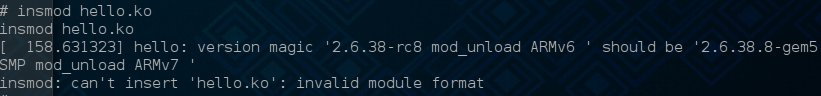
\includegraphics[scale=0.5]{back12.jpg}
	    \end{center}
	    \caption{Inconsistent version magic}
	    \label{fig:vermagic}
	\end{figure}
    Solution: Modify the macro in the /include/linux/vermagic.h
	\begin{figure}[H]
	    \begin{center}
		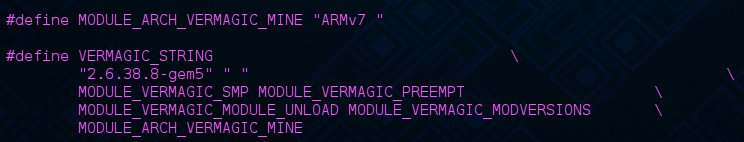
\includegraphics[scale=0.5]{back14.jpg}
	    \end{center}
	    \caption{Modify the version magic}
	    \label{fig:modify}
	\end{figure}
\end{frame}

\begin{frame}
\frametitle{Cont'd}
    Result:
	\begin{figure}[H]
	    \begin{center}
		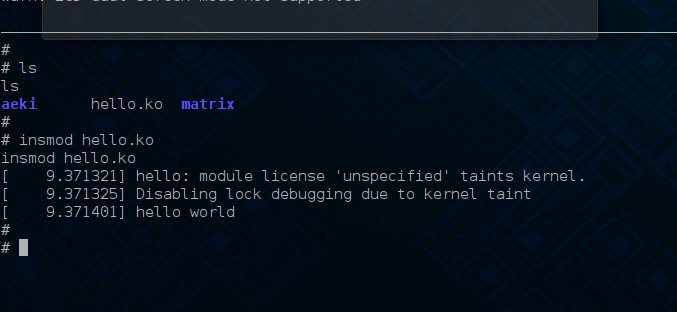
\includegraphics[scale=0.5]{back13.jpg}
	    \end{center}
	    \caption{Successfully inserted the module}
	    \label{fig:hellomodule}
	\end{figure}
\end{frame}
\subsection{A basic character device driver}
\begin{frame}
    \frametitle{A basic character device driver}
A \href{http://www.tldp.org/LDP/lkmpg/2.6/html/lkmpg.html}{simple device driver} that manages read requests.
	\begin{figure}[H]
	    \begin{center}
		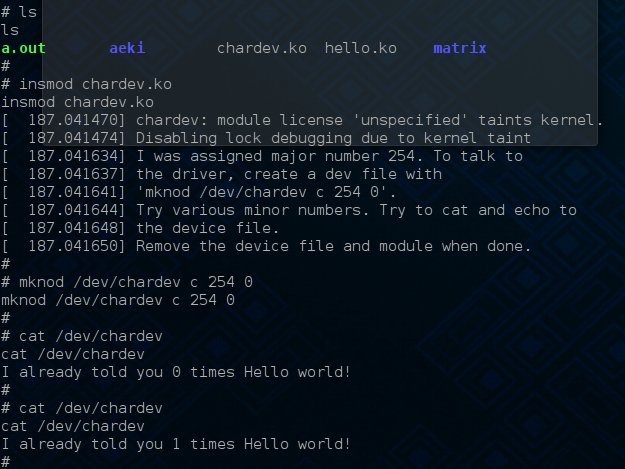
\includegraphics[scale=0.5]{chardev.jpg}
	    \end{center}
	    \caption{A basic character device driver}
	    \label{fig:chardev}
	\end{figure}
    \end{frame}
\section{Running benchmark}
\subsection{Important paths}
\begin{frame}
    \frametitle{Important paths}
\begin{block}{}
    \begin{itemize}
	\item configs/common/SysPaths.py\par
	    Configures the path to kernel and disk image.
	\item configs/common/FSConfig.py\par
	    Configures full-system parameters: memory size,kernel version,etc.
	\item configs/common/Benchmarks.py\par
	    Configures benchmarks.
    \end{itemize}
    \end{block}
	\begin{figure}[H]
	    \begin{center}
		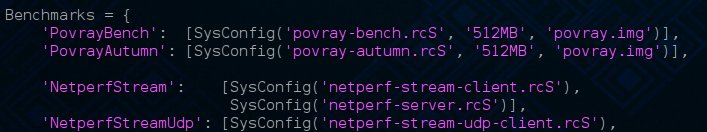
\includegraphics[scale=0.5]{back15.jpg}
	    \end{center}
	    \caption{Benchmarks.py}
	    \label{fig:bench}
	\end{figure}
\end{frame}
\subsection{Shortcut for running benchmarks}
\begin{frame}
    \frametitle{The .rcS file}
    \begin{itemize}
    \item
    The .rcS files are bash scripts for running benchmarks automatically when system starts.
    \item
    The .rcS file resides in configs/boot/. 
    \end{itemize}
    \begin{example}{A typical .rcS file}   
	\lstinputlisting{/home/gyz/code/architecture/fullsys/gem5-stable-fs/configs/boot/gzip.rcS}
    \end{example}
\end{frame}
\begin{frame}
    \frametitle{Register the .rcS file}
	Add an entry to the Benchmarks.py: 	
	\begin{example}
	    'MibenchGSM': [SysConfig('mibench-gsm.rcS','256MB')]
    	\end{example}
	\begin{figure}[H]
	    \begin{center}
		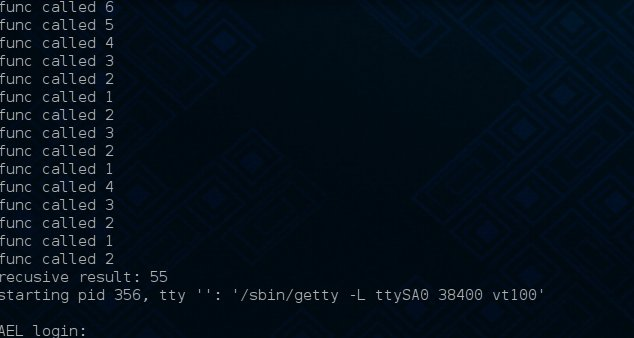
\includegraphics[scale=0.5]{back16.jpg}
	    \end{center}
	    \caption{Run the benchmark automatically}
	    \label{fig:runbench}
	\end{figure}
\end{frame}

\begin{frame}
    \frametitle{Simple Runing Script}
    \begin{itemize}
	\item We could run the benchmarks without invoking the terminal. 
	\item Suitable for batch processing.
    \end{itemize}
    \begin{block}{Script Example}
	\lstinputlisting[firstline=2]{/home/gyz/code/architecture/fullsys/gem5-stable-fs/runAEL-auto.sh}
    \end{block}
\end{frame}
\begin{frame}
    \frametitle{This week's work}
    \begin{itemize}
	\item Study GEM5 source code and kernel module.
	\item Call for ideas.
    \end{itemize}
\end{frame}
\begin{frame}
\Huge{\centerline{Thank you}}
\end{frame}


\end{document} 
